% Options for packages loaded elsewhere
\PassOptionsToPackage{unicode}{hyperref}
\PassOptionsToPackage{hyphens}{url}
%
\documentclass[
]{book}
\usepackage{amsmath,amssymb}
\usepackage{lmodern}
\usepackage{iftex}
\ifPDFTeX
  \usepackage[T1]{fontenc}
  \usepackage[utf8]{inputenc}
  \usepackage{textcomp} % provide euro and other symbols
\else % if luatex or xetex
  \usepackage{unicode-math}
  \defaultfontfeatures{Scale=MatchLowercase}
  \defaultfontfeatures[\rmfamily]{Ligatures=TeX,Scale=1}
\fi
% Use upquote if available, for straight quotes in verbatim environments
\IfFileExists{upquote.sty}{\usepackage{upquote}}{}
\IfFileExists{microtype.sty}{% use microtype if available
  \usepackage[]{microtype}
  \UseMicrotypeSet[protrusion]{basicmath} % disable protrusion for tt fonts
}{}
\makeatletter
\@ifundefined{KOMAClassName}{% if non-KOMA class
  \IfFileExists{parskip.sty}{%
    \usepackage{parskip}
  }{% else
    \setlength{\parindent}{0pt}
    \setlength{\parskip}{6pt plus 2pt minus 1pt}}
}{% if KOMA class
  \KOMAoptions{parskip=half}}
\makeatother
\usepackage{xcolor}
\IfFileExists{xurl.sty}{\usepackage{xurl}}{} % add URL line breaks if available
\IfFileExists{bookmark.sty}{\usepackage{bookmark}}{\usepackage{hyperref}}
\hypersetup{
  pdftitle={Data Management Using R},
  pdfauthor={Myo Minn Oo, MD, PhD},
  hidelinks,
  pdfcreator={LaTeX via pandoc}}
\urlstyle{same} % disable monospaced font for URLs
\usepackage{color}
\usepackage{fancyvrb}
\newcommand{\VerbBar}{|}
\newcommand{\VERB}{\Verb[commandchars=\\\{\}]}
\DefineVerbatimEnvironment{Highlighting}{Verbatim}{commandchars=\\\{\}}
% Add ',fontsize=\small' for more characters per line
\usepackage{framed}
\definecolor{shadecolor}{RGB}{248,248,248}
\newenvironment{Shaded}{\begin{snugshade}}{\end{snugshade}}
\newcommand{\AlertTok}[1]{\textcolor[rgb]{0.94,0.16,0.16}{#1}}
\newcommand{\AnnotationTok}[1]{\textcolor[rgb]{0.56,0.35,0.01}{\textbf{\textit{#1}}}}
\newcommand{\AttributeTok}[1]{\textcolor[rgb]{0.77,0.63,0.00}{#1}}
\newcommand{\BaseNTok}[1]{\textcolor[rgb]{0.00,0.00,0.81}{#1}}
\newcommand{\BuiltInTok}[1]{#1}
\newcommand{\CharTok}[1]{\textcolor[rgb]{0.31,0.60,0.02}{#1}}
\newcommand{\CommentTok}[1]{\textcolor[rgb]{0.56,0.35,0.01}{\textit{#1}}}
\newcommand{\CommentVarTok}[1]{\textcolor[rgb]{0.56,0.35,0.01}{\textbf{\textit{#1}}}}
\newcommand{\ConstantTok}[1]{\textcolor[rgb]{0.00,0.00,0.00}{#1}}
\newcommand{\ControlFlowTok}[1]{\textcolor[rgb]{0.13,0.29,0.53}{\textbf{#1}}}
\newcommand{\DataTypeTok}[1]{\textcolor[rgb]{0.13,0.29,0.53}{#1}}
\newcommand{\DecValTok}[1]{\textcolor[rgb]{0.00,0.00,0.81}{#1}}
\newcommand{\DocumentationTok}[1]{\textcolor[rgb]{0.56,0.35,0.01}{\textbf{\textit{#1}}}}
\newcommand{\ErrorTok}[1]{\textcolor[rgb]{0.64,0.00,0.00}{\textbf{#1}}}
\newcommand{\ExtensionTok}[1]{#1}
\newcommand{\FloatTok}[1]{\textcolor[rgb]{0.00,0.00,0.81}{#1}}
\newcommand{\FunctionTok}[1]{\textcolor[rgb]{0.00,0.00,0.00}{#1}}
\newcommand{\ImportTok}[1]{#1}
\newcommand{\InformationTok}[1]{\textcolor[rgb]{0.56,0.35,0.01}{\textbf{\textit{#1}}}}
\newcommand{\KeywordTok}[1]{\textcolor[rgb]{0.13,0.29,0.53}{\textbf{#1}}}
\newcommand{\NormalTok}[1]{#1}
\newcommand{\OperatorTok}[1]{\textcolor[rgb]{0.81,0.36,0.00}{\textbf{#1}}}
\newcommand{\OtherTok}[1]{\textcolor[rgb]{0.56,0.35,0.01}{#1}}
\newcommand{\PreprocessorTok}[1]{\textcolor[rgb]{0.56,0.35,0.01}{\textit{#1}}}
\newcommand{\RegionMarkerTok}[1]{#1}
\newcommand{\SpecialCharTok}[1]{\textcolor[rgb]{0.00,0.00,0.00}{#1}}
\newcommand{\SpecialStringTok}[1]{\textcolor[rgb]{0.31,0.60,0.02}{#1}}
\newcommand{\StringTok}[1]{\textcolor[rgb]{0.31,0.60,0.02}{#1}}
\newcommand{\VariableTok}[1]{\textcolor[rgb]{0.00,0.00,0.00}{#1}}
\newcommand{\VerbatimStringTok}[1]{\textcolor[rgb]{0.31,0.60,0.02}{#1}}
\newcommand{\WarningTok}[1]{\textcolor[rgb]{0.56,0.35,0.01}{\textbf{\textit{#1}}}}
\usepackage{longtable,booktabs,array}
\usepackage{calc} % for calculating minipage widths
% Correct order of tables after \paragraph or \subparagraph
\usepackage{etoolbox}
\makeatletter
\patchcmd\longtable{\par}{\if@noskipsec\mbox{}\fi\par}{}{}
\makeatother
% Allow footnotes in longtable head/foot
\IfFileExists{footnotehyper.sty}{\usepackage{footnotehyper}}{\usepackage{footnote}}
\makesavenoteenv{longtable}
\usepackage{graphicx}
\makeatletter
\def\maxwidth{\ifdim\Gin@nat@width>\linewidth\linewidth\else\Gin@nat@width\fi}
\def\maxheight{\ifdim\Gin@nat@height>\textheight\textheight\else\Gin@nat@height\fi}
\makeatother
% Scale images if necessary, so that they will not overflow the page
% margins by default, and it is still possible to overwrite the defaults
% using explicit options in \includegraphics[width, height, ...]{}
\setkeys{Gin}{width=\maxwidth,height=\maxheight,keepaspectratio}
% Set default figure placement to htbp
\makeatletter
\def\fps@figure{htbp}
\makeatother
\setlength{\emergencystretch}{3em} % prevent overfull lines
\providecommand{\tightlist}{%
  \setlength{\itemsep}{0pt}\setlength{\parskip}{0pt}}
\setcounter{secnumdepth}{5}
\usepackage{booktabs}
\ifLuaTeX
  \usepackage{selnolig}  % disable illegal ligatures
\fi
\usepackage[]{natbib}
\bibliographystyle{plainnat}

\title{Data Management Using R}
\author{Myo Minn Oo, MD, PhD}
\date{Last updated on 2021-12-12}

\begin{document}
\maketitle

{
\setcounter{tocdepth}{1}
\tableofcontents
}
\hypertarget{section}{%
\chapter*{}\label{section}}
\addcontentsline{toc}{chapter}{}

Welcome to \texttt{dmur}!

This is a book for anyone who are interested in manipulating and processing medical data. This book introduces different aspects of data management and how to implement these in R using RStudio. While there are a plethora of great R books covering a variety of data management topics, I hope this book would serve as a self-learning guide to avoid roadblocks and frustrations before becoming fully comfortable with using R. Many beginners find themselves wanting to develop data management skills in R, but lose their patience after they encounter a steep learning curve of R and several months of frustration. If you feel nostalgic about this, this book is for you.

It is intended for non-technical audience and Stata users to:

\begin{itemize}
\tightlist
\item
  Serve as a guidebook to R code for data management
\item
  Serve as a R code reference manual for \texttt{mStats} package
\item
  Provide task-centered examples addressing common data management problems
\item
  Assist people in transitioning to R
\end{itemize}

\hypertarget{under-construction}{%
\section*{Under construction}\label{under-construction}}
\addcontentsline{toc}{section}{Under construction}

This book is still \textbf{UNDER CONSTRUCTION}. If you have any comments or suggestions, feel free to contact me at \href{mailto::dr.myominnoo@gmail.com}{dr.myominnoo@gmail.com}. Thank you!

if you have a dataset that you think would be suitable for inclusion in this text (as an example or for an exercise), I would love to hear about it.

\hypertarget{inspirations}{%
\section*{Inspirations}\label{inspirations}}
\addcontentsline{toc}{section}{Inspirations}

Tutorials and books that provided ideas and knowledge of this book are credited within their respective pages. More generally, the following sources provided inspiration for this book:

\begin{itemize}
\tightlist
\item
  \href{https://www.stata.com/bookstore/data-management-using-stata/}{Data Management Using Stata: A Practical Handbook}
\item
  \href{https://stats.idre.ucla.edu/stata/}{UCLA's Stata tutorials}
\item
  \href{https://www.epirhandbook.com/en/}{R for applied epidemiology and public health}
\item
  \href{https://r4ds.had.co.nz/}{R for Data Science book (R4DS)}\\
\item
  \href{https://bookdown.org/yihui/bookdown/}{bookdown: Authoring Books and Technical Documents with R Markdown}
\item
  \href{https://www.netlify.com}{Netlify} hosts this website
\end{itemize}

The design of this book is based on the codes obtained from \href{https://github.com/higgi13425/rmrwr-book}{Peter Higgins}. Kudos to Peter!

\hypertarget{how-to-use-this-handbook}{%
\section*{How to use this handbook}\label{how-to-use-this-handbook}}
\addcontentsline{toc}{section}{How to use this handbook}

\begin{itemize}
\tightlist
\item
  Browse the pages in the Table of Contents, or use the search box
\item
  Click the ``copy'' icons to copy code\\
\item
  You can follow along with the example datasets we will download in the next chapter \ref{exampledata}.
\end{itemize}

\hypertarget{software-versions}{%
\section*{Software versions}\label{software-versions}}
\addcontentsline{toc}{section}{Software versions}

The knitr package (Xie 2015) and the bookdown package (Xie 2021) were used to compile this text. The R session information is shown below:

\begin{Shaded}
\begin{Highlighting}[]
\NormalTok{xfun}\SpecialCharTok{::}\FunctionTok{session\_info}\NormalTok{()}
\end{Highlighting}
\end{Shaded}

\begin{verbatim}
## R version 4.1.0 (2021-05-18)
## Platform: x86_64-apple-darwin17.0 (64-bit)
## Running under: macOS Big Sur 10.16
## 
## Locale: en_US.UTF-8 / en_US.UTF-8 / en_US.UTF-8 / C / en_US.UTF-8 / en_US.UTF-8
## 
## Package version:
##   base64enc_0.1.3 bookdown_0.24.4 compiler_4.1.0  digest_0.6.29  
##   evaluate_0.14   fastmap_1.1.0   glue_1.5.1      graphics_4.1.0 
##   grDevices_4.1.0 highr_0.9       htmltools_0.5.2 jquerylib_0.1.4
##   jsonlite_1.7.2  knitr_1.36      magrittr_2.0.1  methods_4.1.0  
##   rlang_0.4.12    rmarkdown_2.11  stats_4.1.0     stringi_1.7.6  
##   stringr_1.4.0   tinytex_0.35    tools_4.1.0     utils_4.1.0    
##   xfun_0.28       yaml_2.2.1
\end{verbatim}

\begin{Shaded}
\begin{Highlighting}[]
\FunctionTok{packageVersion}\NormalTok{(}\StringTok{"tidyverse"}\NormalTok{)}
\end{Highlighting}
\end{Shaded}

\begin{verbatim}
## [1] '1.3.1'
\end{verbatim}

\begin{Shaded}
\begin{Highlighting}[]
\FunctionTok{packageVersion}\NormalTok{(}\StringTok{"dplyr"}\NormalTok{)}
\end{Highlighting}
\end{Shaded}

\begin{verbatim}
## [1] '1.0.7'
\end{verbatim}

\begin{Shaded}
\begin{Highlighting}[]
\FunctionTok{packageVersion}\NormalTok{(}\StringTok{"magrittr"}\NormalTok{)}
\end{Highlighting}
\end{Shaded}

\begin{verbatim}
## [1] '2.0.1'
\end{verbatim}

\begin{Shaded}
\begin{Highlighting}[]
\FunctionTok{packageVersion}\NormalTok{(}\StringTok{"mStats"}\NormalTok{)}
\end{Highlighting}
\end{Shaded}

\begin{verbatim}
## [1] '4.0.0'
\end{verbatim}

\hypertarget{terms-of-use-and-contribution}{%
\section*{Terms of Use and Contribution}\label{terms-of-use-and-contribution}}
\addcontentsline{toc}{section}{Terms of Use and Contribution}

\hypertarget{license}{%
\subsection*{License}\label{license}}
\addcontentsline{toc}{subsection}{License}

Data Management Using R, 2021 This work is licensed by Applied Epi Incorporated under a Creative Commons Attribution-NonCommercial-ShareAlike 4.0 International License.

Academic courses and training programs are welcome to use this handbook with their students, but please send us an email to let me know. If you have questions about your intended use, email \textbf{\href{mailto:dr.myominnoo@gmail.com}{\nolinkurl{dr.myominnoo@gmail.com}}}.

\hypertarget{citation}{%
\subsection*{Citation}\label{citation}}
\addcontentsline{toc}{subsection}{Citation}

Oo, Myo Minn. Data Management Using R. 2021.

\hypertarget{contribution}{%
\subsection*{Contribution}\label{contribution}}
\addcontentsline{toc}{subsection}{Contribution}

If you would like to make a content contribution, please contact with us first via Github issues or by email. We are implementing a schedule for updates and are creating a contributor guide.

Please note that the epiRhandbook project is released with a \href{https://contributor-covenant.org/version/2/0/CODE_OF_CONDUCT.html}{Contributor Code of Conduct}. By contributing to this project, you agree to abide by its terms.

\hypertarget{getting-started}{%
\chapter{Getting Started}\label{getting-started}}

R is an \textbf{free} software for statistics and graphics. It is widely used among statisticians and data scientists for developing statistical software and data analysis.

R is primarily developed in three programming languages: C, Fortan and R itself. Although It itself can be used with command line interface, there are several third-party integrated development environment (IDE) with nice graphical user interface, including RStudio and Jupyter Notebook.

R comes from \texttt{S} programming language. \texttt{S} was created by \href{https://en.wikipedia.org/wiki/John_Chambers_(programmer)}{John Chambers} in 1976 at Bell Labs. Later, two statisticians, Ross Ihaka and Robert Gentleman, developed R that is currently maintained by the R Development Core Team. R is named partly after the first names of the first two R authors and partly as a play on the name of S.

R can be downloaded from \url{http://cran.r-project.org/}.

\hypertarget{rstudio}{%
\section{RStudio}\label{rstudio}}

\texttt{Rstudio} is an integraded environment for R. It comes in two versions: Desktop version is a desktop application and server version runs on a web browser. Regular \texttt{RStudio} for personal usage is free for both desktop and server version.

\begin{quote}
If R is a car engine, then RStudio is the structure of that care, body frame, interior design and every other thing that help us operate it safely, efficiently and comfotably.
\end{quote}

RStudio can be downloaded from \href{https://rstudio.com/products/rstudio/download}{their official website}.

\hypertarget{start-screen}{%
\section{Start screen}\label{start-screen}}

When you open RStudio, you will see a screen that looks like figure \ref{fig:startscreen}.

\begin{figure}
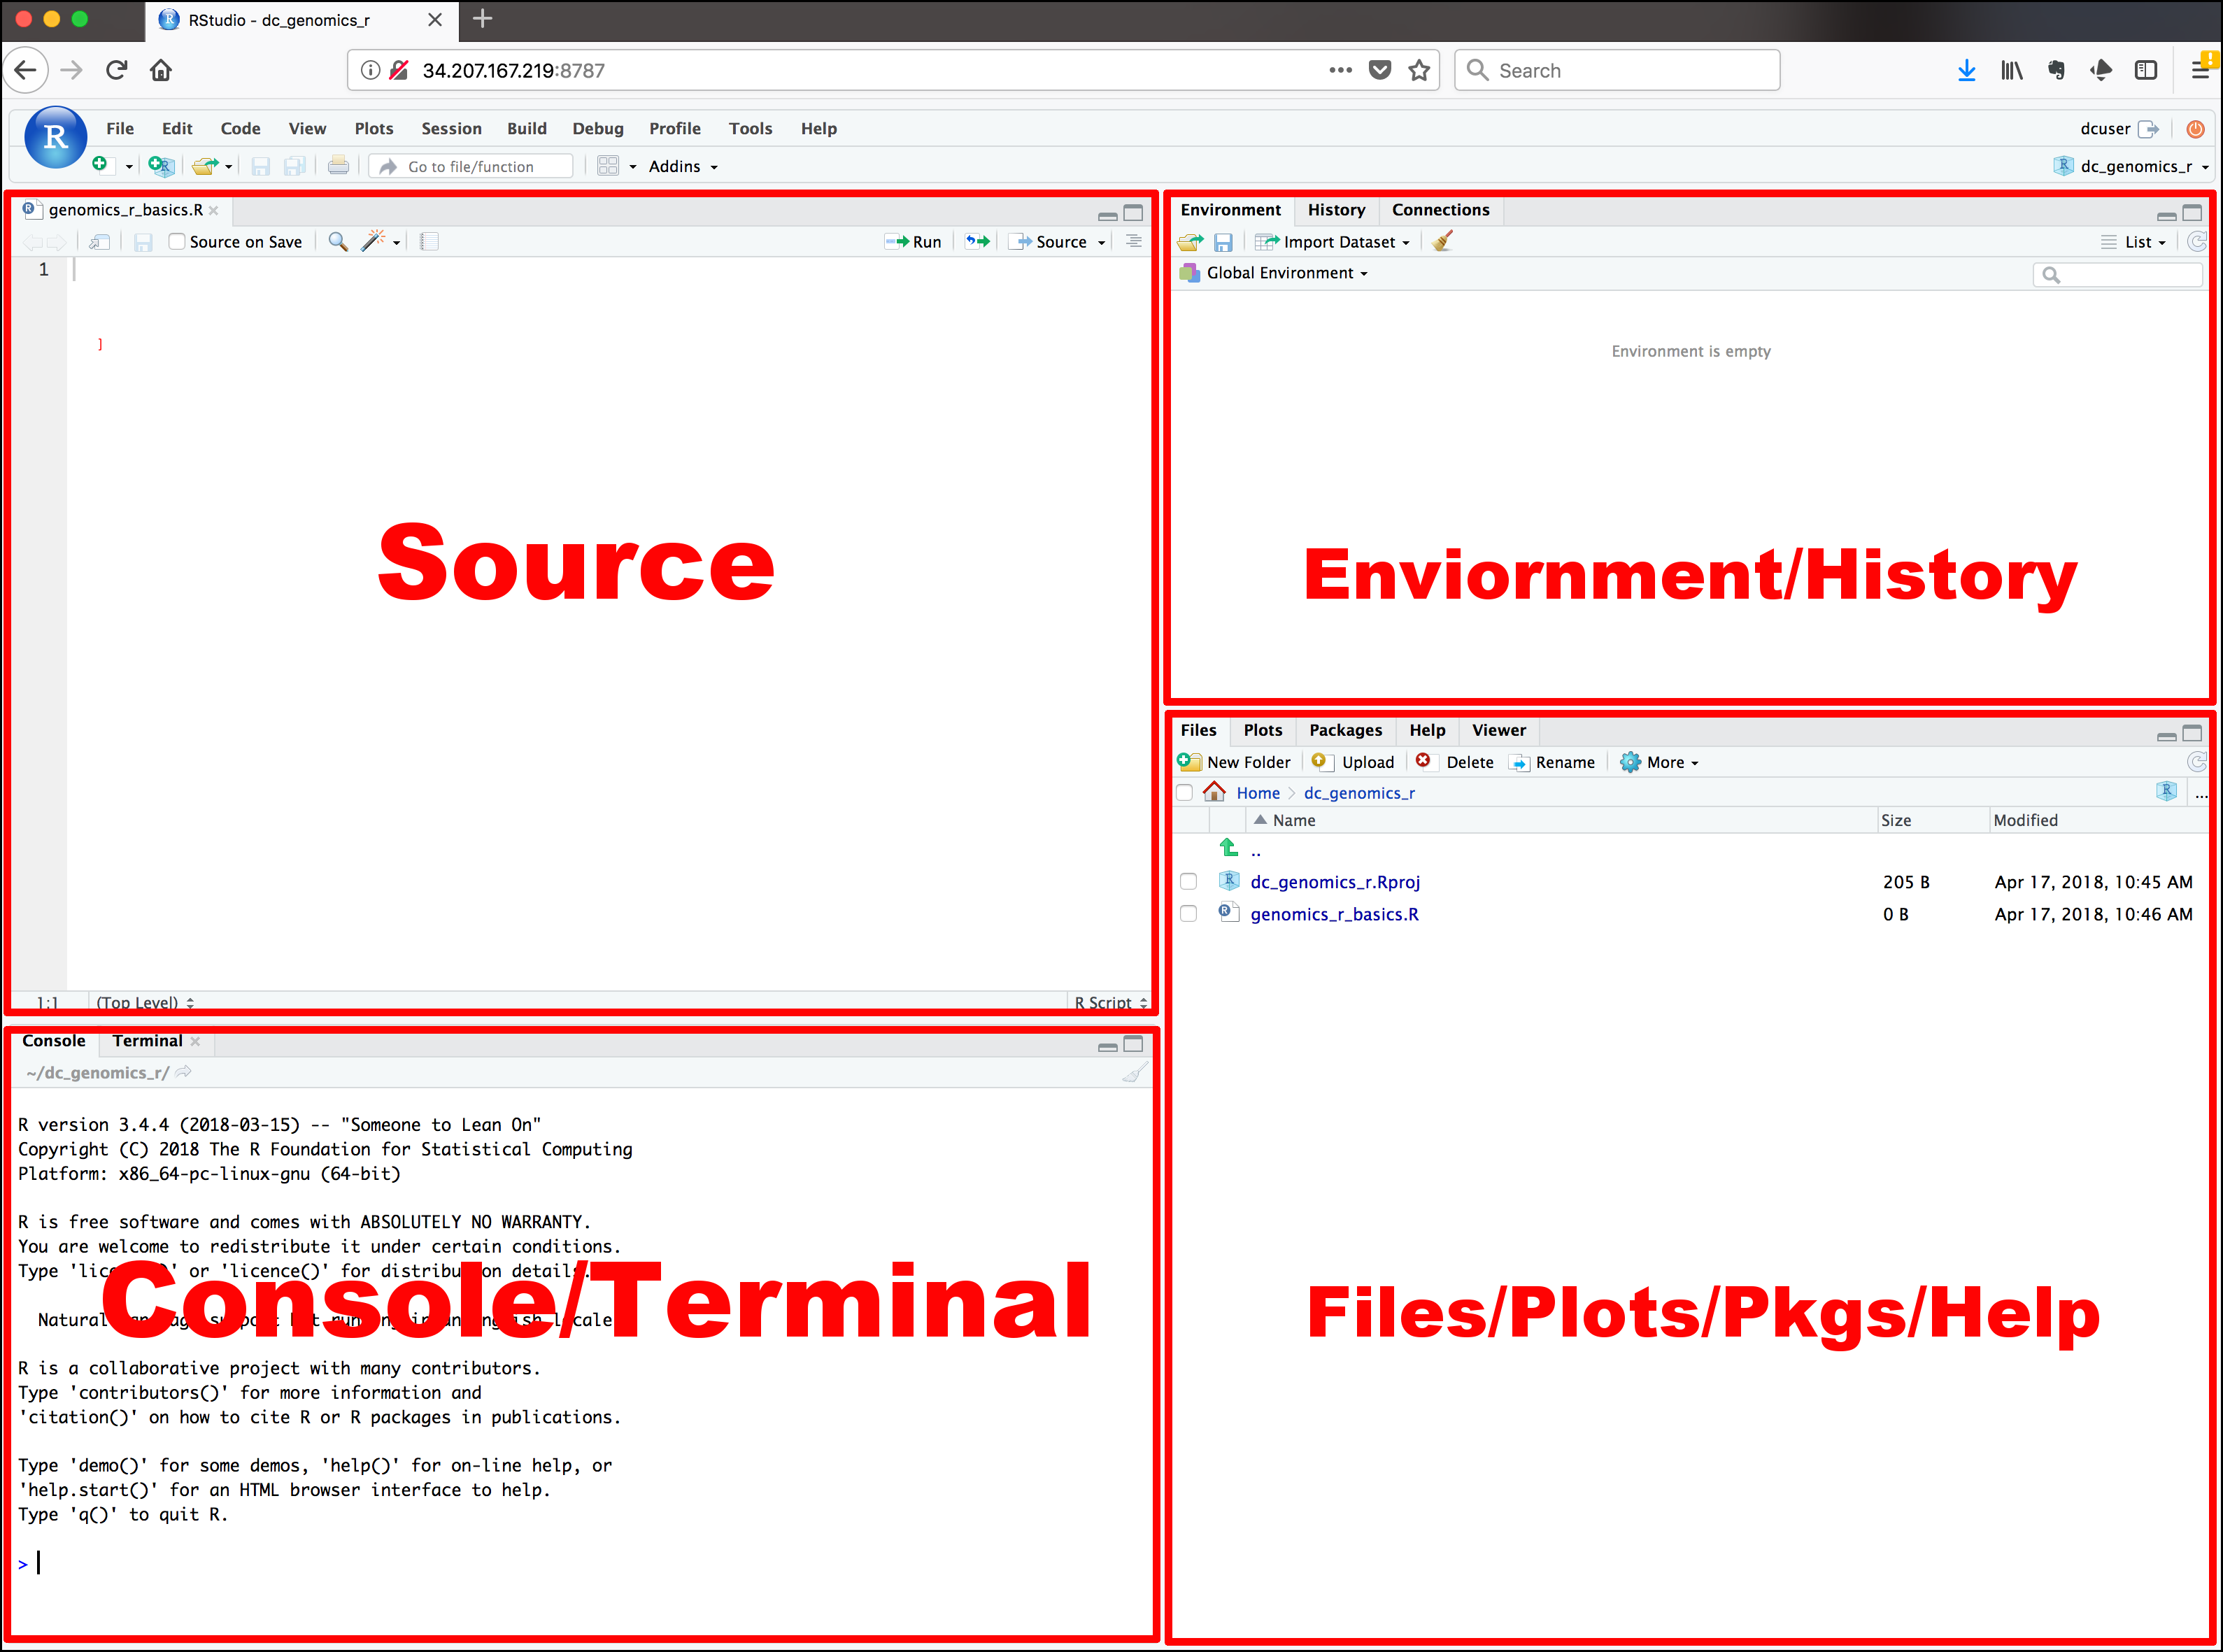
\includegraphics[width=1\linewidth]{img/rstudio_interface} \caption{RStudio's start screen}\label{fig:startscreen}
\end{figure}

The interface has four window panes. Each window pane may have several tabs or sub-windows. By default, \textbf{Source Pane} is on the top-left corner, \textbf{Console Pane} on bottom-left, \textbf{Environment Pane} on top-right, and \textbf{Files Pane} on bottom-right.

\begin{enumerate}
\def\labelenumi{\arabic{enumi}.}
\item
  \textbf{Source Pane} is a text editor that will be referred to as \emph{R Script} later on. You can write commands and save them, which is the main point of reproducibility. Anyone who has this R Script can review and edit it in the future.
\item
  \textbf{Console Pane} is the place you write your line-by-line command. It means you can only write a single command or a long paragraph of commands. After you close the RStudio, the commands will not be saved unless you specified to do so. However, it is the best way to saving \textbf{R Script} in \textbf{Source Pane}to store the commands you desire.

  \begin{itemize}
  \tightlist
  \item
    Symbol \texttt{\textgreater{}} called prompt
  \item
    Type 3 + 4, and press Enter.
  \end{itemize}
\item
  \textbf{Environment Pane} has several sub-windows. For data management and beginner, you only have to know Environment and History.

  \begin{itemize}
  \tightlist
  \item
    \texttt{Environment} is where R works.
  \item
    \texttt{Global\ Environment} is the place where your data will be after importing data.
  \item
    \texttt{History} saves the commands you run in R console.
  \item
    \texttt{Connections} is where you connect to external databases.
  \end{itemize}
\item
  \textbf{Files Pane} also has several sub-windows.

  \begin{itemize}
  \tightlist
  \item
    \texttt{Files} is like a folder manager on your phone. You can manage files and folders as well as set the working directory.
  \item
    \texttt{Plots} is where your plots will appear.
  \item
    \texttt{Packages} is where you manage your R packages. You can install it from CRAN or other repositories. You can also install locally stored R packages.
  \item
    \texttt{Help} is where R stores documentations. You can open the help or introduction page of the respective packages as well as individual functions.
  \end{itemize}
\end{enumerate}

You can arrange these windows as you like. I think putting console on the right upper window will give you a lot of freedom as you will mostly be using \textbf{Source Pane} and \textbf{Console Pane} simultaneously. You can change this by pressing the four window icon below the menu bar and choosing the option \textbf{Console on the Right} as shown in figure \ref{fig:consoleright}.

\begin{figure}

{\centering 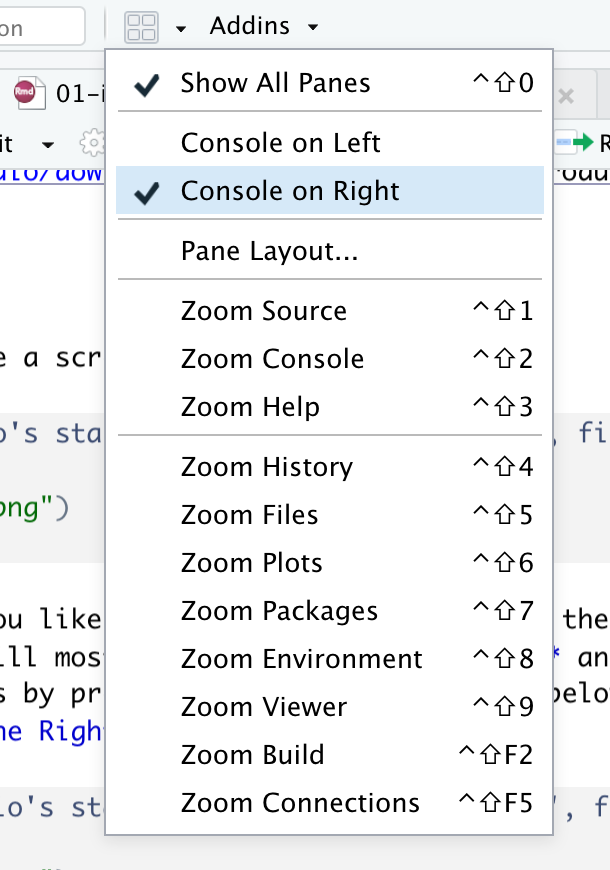
\includegraphics[width=0.5\linewidth]{img/consoleright} 

}

\caption{Changing console to the right upper window}\label{fig:consoleright}
\end{figure}

\hypertarget{r-packages}{%
\section{R Packages}\label{r-packages}}

\texttt{Base\ R} is what you get after installing R. R is powerful because of its tens of thousands of packages. The number is still growing. This also creates the problem of confusion. Even no single user can check or use all packages R can offer. A solution is to stick to certain packages that work well for you. In this book, I will show you a few packages that works for me.

\hypertarget{installing-a-package-from-cran}{%
\subsection{Installing a package from CRAN}\label{installing-a-package-from-cran}}

To install a package, you can use the function \texttt{install.packages("package\_name")} if it is published on \texttt{CRAN}. \texttt{CRAN} is the comprehensive R Archive Network, web servers that store R packages.

Packages installed directly from Github are usually under development, but up-to-date and often free from previous issues and bugs.

Let's install the packages used in this book.

\begin{Shaded}
\begin{Highlighting}[]
\NormalTok{package\_name }\OtherTok{\textless{}{-}} \FunctionTok{c}\NormalTok{(}\StringTok{"tidyverse"}\NormalTok{, }\StringTok{"mStats"}\NormalTok{, }\StringTok{"flextable"}\NormalTok{)}
\FunctionTok{install.packages}\NormalTok{(package\_name)}
\end{Highlighting}
\end{Shaded}

\hypertarget{installing-a-package-from-github}{%
\subsection{Installing a package from GitHub}\label{installing-a-package-from-github}}

For packages published on GitHub, use either \texttt{devtools::install\_github("repo")} or \texttt{remotes::install\_github("repo")}.

Let's illustrate this by installing \texttt{remotes} and then \texttt{mStats} from GitHub.

\begin{Shaded}
\begin{Highlighting}[]
\FunctionTok{install.packages}\NormalTok{(}\StringTok{"remotes"}\NormalTok{)}
\NormalTok{remotes}\SpecialCharTok{::}\FunctionTok{install\_github}\NormalTok{(}\StringTok{"myominnoo/mStats"}\NormalTok{)}
\end{Highlighting}
\end{Shaded}

\hypertarget{essential-packages-for-this-book}{%
\subsection{Essential packages for this book}\label{essential-packages-for-this-book}}

\begin{itemize}
\tightlist
\item
  dplyr
\item
  mStats
\item
  magrittr
\end{itemize}

\hypertarget{mstats}{%
\section{mStats}\label{mstats}}

R has a steep learning curve. For physicians and health professionals, they just want to get started with data management and analysis, rather than spending a lot of time to learn and master R. There might be an advantage to mastering R; however unlike statisticians and programmers, it seems a very daunting process for them to become comfortable with coding in R.

The \texttt{mStats} package was developed to facilitate the data management and analysis in R while requiring only a few basic of R. It takes some principles from one of the most popular statistical software in public health settings, \texttt{STATA}. \texttt{STATA} has been in existence for a long time now that most of its commands are stable, powerful, and intuitive. These features attract power-users and help them accomplish their data tasks.

In a nutshell, \texttt{mStats} is a R package that facilitates data management and analysis of health research in R environment. It includes three core sets of functions that are designed to help data management, data analysis, and reporting streamline for health research projects.

For epidemiology and public health, there are already a number of good packages available for \texttt{R}, including but not limited to \texttt{epiCalc}, \texttt{Epi}, \texttt{epibasix}, \texttt{epiDisplay}, \texttt{epiR} and \texttt{epitools}. \texttt{mStats} does not intend to replace any of them, but to only contribute as much as I can to data management and analysis of health research projects.

\hypertarget{how-it-started}{%
\subsection{How it started}\label{how-it-started}}

The \texttt{mStats} package came into life when I started my doctoral life in Thailand in 2018. The first version of \texttt{mStats} was released in late 2018. Initially it was intended to prove a concept of what I have learnt and how much I could make use of what I have learnt so far. In addition, I would like something open source unlike \texttt{STATA} and something different from base R.

There are two packages that deeply inspired me to do this: \texttt{dplyr} under the universe of \texttt{tidyverse} by \textbf{Hadley Wickham} and \texttt{epiCalc} by my advisor \textbf{Virasakdi Chongsuvivatwong}. The first version of \texttt{mStats} made use of \texttt{ggplot2} and included functions for generating ready-made plots. I released several small patch versions with addition of a few functions that were interesting to me at that time.

In mid 2019, I started another package called \texttt{stats2}. In this package, I tried to simplify the concept of one function doing one task with a few or no options to tweak the task. Although this might be in contrast with the generous flexibility of \texttt{R}, I hardly doubt beginners would mind this limitation. In fact, such simplicity might make users' life easier to get their jobs in R done. The package was on CRAN and released on March 31, 2020.

As times progress, I hope this package will find its way to some people in their works.

\hypertarget{guiding-principles}{%
\subsection{Guiding principles}\label{guiding-principles}}

Most of the guiding principles behind \texttt{dplyr}, \texttt{tidyverse}, and \texttt{STATA} inspire the creation and development of the \texttt{mStats} package:

\begin{itemize}
\item
  \textbf{Compose simple functions with the pipe}:

  \begin{itemize}
  \item
    \texttt{data\ masking} for tidy evaluation: it is very common to use datasets as in the form of \texttt{data\ frame} in as R analysis project. \texttt{R} functions are mostly very generic and created for basic data structures of R. The {[}tidyverse{]} uses tidy evaluation and implements data masking in its \texttt{dplyr} package. This allows manipulation of \textbf{data-variables} as if they were ``programming'' variables that live in an environment. Basically, it allows you to type, as an example, \texttt{generate(airquality,\ lnOzone\ =\ log(Ozone))} instead of \texttt{airquality\$lnOzone\ \textless{}-\ \ log(airquality\$Ozone)}.
  \item
    The principle of pipes changes the paradigm of coding in \texttt{R}. The use of the pipe function \texttt{\%\textgreater{}\%} from the \texttt{magrittr} package allows for cleaner code and enhances readability of the codes. Most functions in \texttt{mStats} is compatible with the usage of the pipe function.
  \end{itemize}
\item
  \textbf{Designed for humans}:

  \begin{itemize}
  \item
    \texttt{KISS}: Keep \texttt{functions} short and simple - one function does only one task with few options to change the nature of the task. \texttt{mStats} intentionally limits options of arguments in functions and attempts to balance between having too many argument options and having no options at all.
  \item
    \texttt{Labels}: \texttt{mStats} consistently uses the concept of \textbf{labelling variables and datasets}. It also streamlines \texttt{labels} for the purpose of report generation. Though it is not necessary to label values, this can be done using certain packages like \texttt{labelled} and \texttt{sjlabelled}.
  \item
    Outputs: outputs in the console are well-formatted for the ease of interpretation.
  \end{itemize}
\item
  \textbf{Reproducible research}

  \begin{itemize}
  \tightlist
  \item
    Making tables is One of the most common tasks in health research analysis where most researchers waste much time. Reproducibility in health research is becoming crucially important and depends on streamlining this process. \texttt{mStats} provides one of many workflows used for tables generation and link to \texttt{R} codes for getting the job done.
  \end{itemize}
\end{itemize}

\hypertarget{package-masking}{%
\section{Package masking}\label{package-masking}}

Packages including \texttt{mStats} might contain functions that are in conflicts with other packages. I suggest to explicitly use the syntax to call the desired package, \texttt{package::function}.

For example, the \texttt{cut} function from \texttt{mStats} will be masked from the \texttt{cut} function from \texttt{base}. When you want to use the function from base, you need to write this: \texttt{base::cut()}.

\hypertarget{piping-your-workflow}{%
\section{Piping your workflow}\label{piping-your-workflow}}

The pipe function \texttt{\%\textgreater{}\%} from the \texttt{magrittr} package can connect several lines of codes in a single workflow. It allows cleaner codes and enhances human readability. As an example, if you have three generic functions, you can write codes like this: \texttt{function3(function32(function31(...,\ data),\ ...),\ ...)}. But it is confusing. By using \texttt{\%\textgreater{}\%}, we can arrange codes from top to bottom and left to right as follow:

\begin{Shaded}
\begin{Highlighting}[]
\NormalTok{data }\SpecialCharTok{\%\textgreater{}\%}
  \FunctionTok{function1}\NormalTok{(...) }\SpecialCharTok{\%\textgreater{}\%} 
  \FunctionTok{function2}\NormalTok{(...) }\SpecialCharTok{\%\textgreater{}\%} 
  \FunctionTok{function3}\NormalTok{(...)}
\end{Highlighting}
\end{Shaded}

\hypertarget{searching-help}{%
\section{Searching Help}\label{searching-help}}

\hypertarget{general}{%
\subsection{General}\label{general}}

If you get stuck, try to google it or search on virtual forums like \texttt{Stack\ Overflow}. Most of what you want to know are already answered or solved in one of those forums.

\hypertarget{getting-help}{%
\subsection{Getting help}\label{getting-help}}

If you encounter a clear bug, please file an issue with a minimal
reproducible example on
\href{https://github.com/myominnoo/mStats/issues}{GitHub}. For questions and
other discussion, please directly email me \href{mailto::dr.myominnoo@gmail.com}{dr.myominnoo@gmail.com} or use the \href{https://groups.google.com/g/mstats}{mStats mailing list}.

\hypertarget{exampledata}{%
\section{Example datasets}\label{exampledata}}

In this book, we will use datasets from several sources. The code chunks below download these datasets into a \texttt{data} folder under your current working directory.

Let's create a function that takes a URL link for zipped files, download, and unzip the files into specified directory.

\begin{Shaded}
\begin{Highlighting}[]
\NormalTok{download\_zipfile }\OtherTok{\textless{}{-}} \ControlFlowTok{function}\NormalTok{(url, }\AttributeTok{exdir =} \StringTok{"data/"}\NormalTok{, }\AttributeTok{file =} \FunctionTok{tempfile}\NormalTok{(), }\AttributeTok{junkpaths =} \ConstantTok{TRUE}\NormalTok{) \{}
    \ControlFlowTok{for}\NormalTok{ (link }\ControlFlowTok{in}\NormalTok{ url) \{}
        \DocumentationTok{\#\# download the dmus2 zipped file into temporary file}
        \FunctionTok{download.file}\NormalTok{(link, file)}
        
        \DocumentationTok{\#\# extract the dmus2 datasets into the data folder}
        \FunctionTok{unzip}\NormalTok{(file, }\AttributeTok{exdir =}\NormalTok{ exdir, }\AttributeTok{junkpaths =} \ConstantTok{TRUE}\NormalTok{)}
\NormalTok{    \}}
\NormalTok{\}}
\end{Highlighting}
\end{Shaded}

\hypertarget{dmus2}{%
\subsection{dmus2}\label{dmus2}}

The following code chunk downloads datasets from one of the most popular data management books for Stata, \href{https://www.stata-press.com/data/dmus2.html}{Data Management Using Stata: A Practical Handbook, Second Edition}

\begin{Shaded}
\begin{Highlighting}[]
\DocumentationTok{\#\# Download dmus2 zipped file}
\FunctionTok{download\_zipfile}\NormalTok{(}\StringTok{"https://www.stata{-}press.com/data/dmus2/dmus2.zip"}\NormalTok{, }
                 \AttributeTok{exdir =} \StringTok{"data/dmus2"}\NormalTok{)}
\end{Highlighting}
\end{Shaded}

\hypertarget{who-mortality-data}{%
\subsection{WHO Mortality Data}\label{who-mortality-data}}

THe following code chunks download datasets from \href{https://www.who.int/data/data-collection-tools/who-mortality-database}{WHO webpage}.

\begin{Shaded}
\begin{Highlighting}[]
\DocumentationTok{\#\# 1. A list of countries{-}years available for the mortality and population data.}
\DocumentationTok{\#\# 2. Reference populations and live births.}
\DocumentationTok{\#\# 3. Country codes}
\NormalTok{file }\OtherTok{\textless{}{-}} \FunctionTok{c}\NormalTok{(}\StringTok{"https://cdn.who.int/media/docs/default{-}source/world{-}health{-}data{-}platform/mortality{-}raw{-}data/mort\_availability.zip?sfvrsn=23261e11\_15\&ua=1"}\NormalTok{, }
          \StringTok{"https://cdn.who.int/media/docs/default{-}source/world{-}health{-}data{-}platform/mortality{-}raw{-}data/mort\_pop.zip?sfvrsn=937039fc\_10\&ua=1"}\NormalTok{, }
          \StringTok{"https://cdn.who.int/media/docs/default{-}source/world{-}health{-}data{-}platform/mortality{-}raw{-}data/mort\_country\_codes.zip?sfvrsn=800faac2\_5\&ua=1"}\NormalTok{)}
\FunctionTok{download\_zipfile}\NormalTok{(file, }\AttributeTok{exdir =} \StringTok{"data/who"}\NormalTok{)}
\end{Highlighting}
\end{Shaded}

\hypertarget{ucla-stata-tutorial}{%
\subsection{UCLA Stata Tutorial}\label{ucla-stata-tutorial}}

The following code chunks download datasets from \href{}{UCLA's Stata tutorials}.

\begin{Shaded}
\begin{Highlighting}[]
\ControlFlowTok{if}\NormalTok{ (}\SpecialCharTok{!}\FunctionTok{dir.exists}\NormalTok{(}\StringTok{"data/ucla"}\NormalTok{)) }
    \FunctionTok{dir.create}\NormalTok{(}\StringTok{"data/ucla"}\NormalTok{) }\DocumentationTok{\#\# this will create a directory if it\textquotesingle{}s not there}

\FunctionTok{download.file}\NormalTok{(}\StringTok{"http://stats.idre.ucla.edu/stat/data/patient\_pt1\_stata\_dm.dta"}\NormalTok{, }
              \AttributeTok{destfile =} \StringTok{"data/ucla/patient\_pt1\_stata\_dm.dta"}\NormalTok{)}
\FunctionTok{download.file}\NormalTok{(}\StringTok{"http://stats.idre.ucla.edu/stat/data/patient\_pt2\_stata\_dm.dta"}\NormalTok{, }
              \AttributeTok{destfile =} \StringTok{"data/ucla/patient\_pt2\_stata\_dm.dta"}\NormalTok{)}
\FunctionTok{download.file}\NormalTok{(}\StringTok{"http://stats.idre.ucla.edu/stat/data/doctor\_stata\_dm.dta"}\NormalTok{, }
              \AttributeTok{destfile =} \StringTok{"data/ucla/doctor\_stata\_dm.dta"}\NormalTok{)}

\FunctionTok{download.file}\NormalTok{(}\StringTok{"http://stats.idre.ucla.edu/stat/data/hsb2.csv"}\NormalTok{, }
              \AttributeTok{destfile =} \StringTok{"data/ucla/hsb2.csv"}\NormalTok{)}
\FunctionTok{download.file}\NormalTok{(}\StringTok{"http://stats.idre.ucla.edu/stat/data/hsb2.xls"}\NormalTok{, }
              \AttributeTok{destfile =} \StringTok{"data/ucla/hsb2.xls"}\NormalTok{)}
\end{Highlighting}
\end{Shaded}

\hypertarget{miliary-tuberculosis}{%
\subsection{Miliary Tuberculosis}\label{miliary-tuberculosis}}

The following dataset was used to evaluated a scoring system for central nervous tuberculosis among patients with miliary tuberculosis in a Chinese hospital. Read their study \href{https://journals.plos.org/plosone/article?id=10.1371/journal.pone.0176651}{here}.

We put this dataset into a separate path \texttt{data/others/}.

\begin{Shaded}
\begin{Highlighting}[]
\ControlFlowTok{if}\NormalTok{ (}\SpecialCharTok{!}\FunctionTok{dir.exists}\NormalTok{(}\StringTok{"data/others"}\NormalTok{)) }
    \FunctionTok{dir.create}\NormalTok{(}\StringTok{"data/others"}\NormalTok{) }\DocumentationTok{\#\# this will create a directory if it\textquotesingle{}s not there}

\FunctionTok{download.file}\NormalTok{(}\StringTok{"https://journals.plos.org/plosone/article/file?type=supplementary\&id=info:doi/10.1371/journal.pone.0176651.s001"}\NormalTok{, }
              \AttributeTok{destfile =} \StringTok{"data/others/miliary\_tb.xlsx"}\NormalTok{)}
\end{Highlighting}
\end{Shaded}

\hypertarget{using-existing-data-files}{%
\chapter{Using existing data files}\label{using-existing-data-files}}

You have some data that you are eager to analyze using R. Before you can analyze the data, you must first read the data into R. This chapter describes how you can read common types of data files into R.

\hypertarget{working-directories}{%
\section{Working directories}\label{working-directories}}

I would recommend against using absolute pathway with the \texttt{setwd()} function for your works. One main reason is that other people don't have the same pathways as yours, and it makes replicating codes in other people's devices extremely cumbersome. There are two ways I find more efficient and productive than just setting up your directory with \texttt{setwd()}.

\begin{enumerate}
\def\labelenumi{\arabic{enumi}.}
\tightlist
\item
  Open RStudio by doublie-clicking the \texttt{.R} file.
\item
  Create an R project and open RStudio by double-clicking the \texttt{.Rproj} file.
\end{enumerate}

Both methods will automatically set up your working directory to the folder where your \texttt{.R} or \texttt{.Rproj} file exists. Then you use relative pathway to navigate to other folders and files.

If you have followed the section on downloading \texttt{dmus2} datasets, you might already have a \texttt{data} folder. You can put this data folder under your project folder, whatever you may call it. For the sake of demonstration, let's create a folder named \texttt{dmur} and put this \texttt{data} folder under \texttt{dmur}. You can start create necessary \texttt{.R} and \texttt{.Rproj} files as follows. Essentially, you will have the following structures under the\texttt{dmur} folder.

\begin{Shaded}
\begin{Highlighting}[]
\SpecialCharTok{{-}}\NormalTok{ dmur              }\DocumentationTok{\#\# this is your project or root folder}
    \SpecialCharTok{|}
    \SpecialCharTok{{-}}\NormalTok{ data          }\DocumentationTok{\#\# this is data folder that contains \textasciigrave{}dmus2\textasciigrave{} datasets.}
        \SpecialCharTok{|}
        \SpecialCharTok{{-}}\NormalTok{ many datasets ...     }\DocumentationTok{\#\# these are \textasciigrave{}dmus2\textasciigrave{} datasets}

    \SpecialCharTok{|}
    \SpecialCharTok{{-}}\NormalTok{ dmur.R  }\DocumentationTok{\#\# You can double{-}click this to open RStudio }
    \SpecialCharTok{|}
    \SpecialCharTok{{-}}\NormalTok{ dmur.Rproj  }\DocumentationTok{\#\# You can also double{-}click this to open RStudio}
\end{Highlighting}
\end{Shaded}

{[}To add how to create .R or .Rproj files{]}

\hypertarget{reading-data-files-into-r}{%
\section{Reading data files into R}\label{reading-data-files-into-r}}

There are several data files that you can read and import into R. This chapter begins by illustrating how you can read several common types of datasets into R. As you would expect, you can certainly do this in multiple ways; however I will show the ways I think simplest and most efficient.

In previous section \ref{exampledata}, we have downloaded several datasets into respective folders under a \texttt{data} folder of your current working directory. It should look like the following structure.

\begin{Shaded}
\begin{Highlighting}[]
\SpecialCharTok{{-}}\NormalTok{ Your current working directory}
    \SpecialCharTok{|}
\NormalTok{    \_ data}
        \SpecialCharTok{|}
\NormalTok{        \_ dmus2     }\DocumentationTok{\#\# \textless{}\textless{}== This is where dmus2 datasets were downloaded ==\textgreater{}\textgreater{} }
        \SpecialCharTok{|}
\NormalTok{        \_ who       }\DocumentationTok{\#\# \textless{}\textless{}== This is where who datasets were downloaded ==\textgreater{}\textgreater{}}
\end{Highlighting}
\end{Shaded}

When we specify a path later, we will use this folder structure. If we want to import a dataset from \texttt{dmus2} folder, we will specify the file in this format \texttt{./data/dmus2/filename}.

\hypertarget{csv-and-text-data-files}{%
\subsection{CSV and text data files}\label{csv-and-text-data-files}}

Comma-separated values files, also known as \texttt{CSV} files, are a common format for storing raw data. They have a filename extension of \texttt{.csv}. As the name suggests, \texttt{CSV} files use \texttt{commas} to separate the variables (columns) of the data. Data files in \texttt{CSV} format often include the names of the variables in the first row, also separated by commas.

We illustrate this below by using a \texttt{momkid1.csv} data file, which includes identification number of mom, month, day and year of mom's birthday, and kid's birthday.

While there are several ways to import a raw data file, we use \texttt{read\_csv()} function from the \texttt{readr} package. As we use this function probably once at this time when we import datasets, we write \texttt{readr::read\_csv()} to indicate the function from \texttt{readr} package without loading the whole package. We will use this pattern in the whole book whenever we need one particular function from a package at one time.

\begin{Shaded}
\begin{Highlighting}[]
\NormalTok{momkid1 }\OtherTok{\textless{}{-}}\NormalTok{ readr}\SpecialCharTok{::}\FunctionTok{read\_csv}\NormalTok{(}\StringTok{"data/dmus2/momkid1.csv"}\NormalTok{)}
\end{Highlighting}
\end{Shaded}

\begin{verbatim}
## Rows: 4 Columns: 5
\end{verbatim}

\begin{verbatim}
## -- Column specification --------------------------------------------------------
## Delimiter: ","
## chr (1): kidbday
## dbl (4): momid, momm, momd, momy
\end{verbatim}

\begin{verbatim}
## 
## i Use `spec()` to retrieve the full column specification for this data.
## i Specify the column types or set `show_col_types = FALSE` to quiet this message.
\end{verbatim}

\begin{Shaded}
\begin{Highlighting}[]
\NormalTok{momkid1}
\end{Highlighting}
\end{Shaded}

\begin{verbatim}
## # A tibble: 4 x 5
##   momid  momm  momd  momy kidbday  
##   <dbl> <dbl> <dbl> <dbl> <chr>    
## 1     1    11    28  1972 1/5/1998 
## 2     2     4     3  1973 4/11/2002
## 3     3     6    13  1968 5/15/1996
## 4     4     1     5  1960 1/4/2004
\end{verbatim}

The imported dataset can be displayed in the console just by typing in the assigned object name \texttt{momkid1}.

Text files are also quite popular in storing simple raw data. In the example below, the \texttt{dentists1.txt} data file contains five rows of data regarding five dentists. The four variables reflect the name of the dentist, the years she or he has been practicing, whether she or he works full time, and whether she or he recommends Quaddent gum.

\begin{Shaded}
\begin{Highlighting}[]
\NormalTok{dentists1 }\OtherTok{\textless{}{-}}\NormalTok{ readr}\SpecialCharTok{::}\FunctionTok{read\_csv}\NormalTok{(}\StringTok{"data/dmus2/dentists1.txt"}\NormalTok{)}
\end{Highlighting}
\end{Shaded}

\begin{verbatim}
## Rows: 5 Columns: 4
\end{verbatim}

\begin{verbatim}
## -- Column specification --------------------------------------------------------
## Delimiter: ","
## chr (1): name
## dbl (3): years, fulltime, recom
\end{verbatim}

\begin{verbatim}
## 
## i Use `spec()` to retrieve the full column specification for this data.
## i Specify the column types or set `show_col_types = FALSE` to quiet this message.
\end{verbatim}

\begin{Shaded}
\begin{Highlighting}[]
\NormalTok{dentists1}
\end{Highlighting}
\end{Shaded}

\begin{verbatim}
## # A tibble: 5 x 4
##   name              years fulltime recom
##   <chr>             <dbl>    <dbl> <dbl>
## 1 Y. Don Uflossmore  7.25        0     1
## 2 Olive Tu'Drill    10.2         1     1
## 3 Isaac O'Yerbreath 32.8         1     1
## 4 Ruth Canaale      22           1     1
## 5 Mike Avity         8.5         0     0
\end{verbatim}

See \texttt{?read\_csv} for more details on their optional arguments.

\hypertarget{exercises}{%
\subsubsection{Exercises}\label{exercises}}

We have downloaded a few mortality datasets from WHO. Try to import the following datasets without looking at the answer:

\begin{itemize}
\tightlist
\item
  \texttt{pop} which contains reference population* and live birth data.
\item
  \texttt{country\_codes} which contains country codes
\end{itemize}

\hypertarget{solutions}{%
\subsubsection{Solutions}\label{solutions}}

As you might realize, there is no file extension for these files. Try opening these files with a text editor. You will see that these files are stored in comma-separated format. Hence, we will read using \texttt{readr::read\_csv()}

\begin{Shaded}
\begin{Highlighting}[]
\NormalTok{pop }\OtherTok{\textless{}{-}}\NormalTok{ readr}\SpecialCharTok{::}\FunctionTok{read\_csv}\NormalTok{(}\StringTok{"data/who/pop"}\NormalTok{)}
\end{Highlighting}
\end{Shaded}

\begin{verbatim}
## Rows: 9719 Columns: 33
\end{verbatim}

\begin{verbatim}
## -- Column specification --------------------------------------------------------
## Delimiter: ","
## chr  (2): SubDiv, Frmat
## dbl (31): Country, Admin1, Year, Sex, Pop1, Pop2, Pop3, Pop4, Pop5, Pop6, Po...
\end{verbatim}

\begin{verbatim}
## 
## i Use `spec()` to retrieve the full column specification for this data.
## i Specify the column types or set `show_col_types = FALSE` to quiet this message.
\end{verbatim}

\begin{Shaded}
\begin{Highlighting}[]
\NormalTok{pop}
\end{Highlighting}
\end{Shaded}

\begin{verbatim}
## # A tibble: 9,719 x 33
##    Country Admin1 SubDiv  Year   Sex Frmat    Pop1   Pop2   Pop3  Pop4  Pop5
##      <dbl>  <dbl> <chr>  <dbl> <dbl> <chr>   <dbl>  <dbl>  <dbl> <dbl> <dbl>
##  1    1060     NA <NA>    1980     1 07     137100   3400  15800    NA    NA
##  2    1060     NA <NA>    1980     2 07     159000   4000  18400    NA    NA
##  3    1125     NA <NA>    1955     1 02    5051500 150300 543400    NA    NA
##  4    1125     NA <NA>    1955     2 02    5049400 145200 551000    NA    NA
##  5    1125     NA <NA>    1956     1 02    5353700 158700 576600    NA    NA
##  6    1125     NA <NA>    1956     2 02    5351400 153600 584800    NA    NA
##  7    1125     NA <NA>    1957     1 02    5403000 160300 580800    NA    NA
##  8    1125     NA <NA>    1957     2 02    5392000 155300 589400    NA    NA
##  9    1125     NA <NA>    1958     1 02    5506900 162800 592000    NA    NA
## 10    1125     NA <NA>    1958     2 02    5494400 157800 600100    NA    NA
## # ... with 9,709 more rows, and 22 more variables: Pop6 <dbl>, Pop7 <dbl>,
## #   Pop8 <dbl>, Pop9 <dbl>, Pop10 <dbl>, Pop11 <dbl>, Pop12 <dbl>, Pop13 <dbl>,
## #   Pop14 <dbl>, Pop15 <dbl>, Pop16 <dbl>, Pop17 <dbl>, Pop18 <dbl>,
## #   Pop19 <dbl>, Pop20 <dbl>, Pop21 <dbl>, Pop22 <dbl>, Pop23 <dbl>,
## #   Pop24 <dbl>, Pop25 <dbl>, Pop26 <dbl>, Lb <dbl>
\end{verbatim}

\begin{Shaded}
\begin{Highlighting}[]
\NormalTok{country\_codes }\OtherTok{\textless{}{-}}\NormalTok{ readr}\SpecialCharTok{::}\FunctionTok{read\_csv}\NormalTok{(}\StringTok{"data/who/country\_codes"}\NormalTok{)}
\end{Highlighting}
\end{Shaded}

\begin{verbatim}
## Rows: 227 Columns: 2
\end{verbatim}

\begin{verbatim}
## -- Column specification --------------------------------------------------------
## Delimiter: ","
## chr (1): name
## dbl (1): country
\end{verbatim}

\begin{verbatim}
## 
## i Use `spec()` to retrieve the full column specification for this data.
## i Specify the column types or set `show_col_types = FALSE` to quiet this message.
\end{verbatim}

\begin{Shaded}
\begin{Highlighting}[]
\NormalTok{country\_codes}
\end{Highlighting}
\end{Shaded}

\begin{verbatim}
## # A tibble: 227 x 2
##    country name                    
##      <dbl> <chr>                   
##  1    1010 Algeria                 
##  2    1020 Angola                  
##  3    1025 Benin                   
##  4    1030 Botswana                
##  5    1035 Burkina Faso            
##  6    1040 Burundi                 
##  7    1045 Cameroon                
##  8    1060 Cape Verde              
##  9    1070 Central African Republic
## 10    1080 Chad                    
## # ... with 217 more rows
\end{verbatim}

\hypertarget{excel-spreadsheets}{%
\subsection{Excel spreadsheets}\label{excel-spreadsheets}}

You frequently receive data files stored as Excel spreadsheets. For example, the spreadsheet file named \texttt{dentists.xls} contains information about five dentists. You can import Excel spreadsheets into R by using \texttt{read\_excel()} from the \texttt{readxl} package.

\begin{Shaded}
\begin{Highlighting}[]
\NormalTok{dentists }\OtherTok{\textless{}{-}}\NormalTok{ readxl}\SpecialCharTok{::}\FunctionTok{read\_excel}\NormalTok{(}\StringTok{"data/dmus2/dentists.xls"}\NormalTok{)}
\NormalTok{dentists}
\end{Highlighting}
\end{Shaded}

\begin{verbatim}
## # A tibble: 5 x 4
##   name              years fulltime recom
##   <chr>             <dbl>    <dbl> <dbl>
## 1 Y. Don Uflossmore  7.25        0     1
## 2 Olive Tu'Drill    10.2         1     1
## 3 Isaac O'Yerbreath 32.8         1     1
## 4 Ruth Canaale      22           1     1
## 5 Mike Avity         8.5         0     0
\end{verbatim}

As we did with \texttt{dentists.xls}, let's import another file named \texttt{dentists2.xls} using the \texttt{read\_excel()} function.

\begin{Shaded}
\begin{Highlighting}[]
\NormalTok{dentists2 }\OtherTok{\textless{}{-}}\NormalTok{ readxl}\SpecialCharTok{::}\FunctionTok{read\_excel}\NormalTok{(}\StringTok{"data/dmus2/dentists2.xls"}\NormalTok{)}
\NormalTok{dentists2}
\end{Highlighting}
\end{Shaded}

\begin{verbatim}
## # A tibble: 4 x 2
##   name       years
##   <chr>      <dbl>
## 1 I. Sue Yoo     3
## 2 A. Dewey       8
## 3 B. Cheetem    11
## 4 C. Howe       21
\end{verbatim}

Only 2 variables and 4 observations were imported. These are the names of lawyers. If you open the file with Excel or a spreadsheet program, you will realize that there are three sheets in the file, namely \texttt{lawyers}, \texttt{dentists}, and \texttt{Sheet2}. When there are multiple sheets in an Excel file, the default behavior for the \texttt{read\_excel()} function is to import the first sheet. As such, the results from the list command above is showing a listing of lawyers because the first sheet contained information about lawyers.

We can import the contents of the sheet named \texttt{dentists} by adding the optional argument \texttt{sheet\ =\ "dentists"}, as illustrated below. This tells the function that it should specifically import the sheet named \texttt{dentists}.

\begin{Shaded}
\begin{Highlighting}[]
\NormalTok{dentists2 }\OtherTok{\textless{}{-}}\NormalTok{ readxl}\SpecialCharTok{::}\FunctionTok{read\_excel}\NormalTok{(}\StringTok{"data/dmus2/dentists2.xls"}\NormalTok{, }\AttributeTok{sheet =} \StringTok{"dentists"}\NormalTok{)}
\NormalTok{dentists2}
\end{Highlighting}
\end{Shaded}

\begin{verbatim}
## # A tibble: 5 x 4
##   name              years fulltime recom
##   <chr>             <dbl>    <dbl> <dbl>
## 1 Y. Don Uflossmore  7.25        0     1
## 2 Olive Tu'Drill    10.2         1     1
## 3 Isaac O'Yerbreath 32.8         1     1
## 4 Ruth Canaale      22           1     1
## 5 Mike Avity         8.5         0     0
\end{verbatim}

As we would expect, the imported dataset has 4 variables and 5 observations which matches the contents of the \texttt{dentists} sheet.

Another file named \texttt{dentist3.xls} has additional information stored along with the data. In particular, column E contains notes about the dentists, and the last row, row 7, contains column totals for some of the variables. Let's try to import this excel file using \texttt{read\_excel()}.

\begin{Shaded}
\begin{Highlighting}[]
\NormalTok{dentists3 }\OtherTok{\textless{}{-}}\NormalTok{ readxl}\SpecialCharTok{::}\FunctionTok{read\_excel}\NormalTok{(}\StringTok{"data/dmus2/dentists3.xls"}\NormalTok{)}
\end{Highlighting}
\end{Shaded}

\begin{verbatim}
## New names:
## * `` -> ...5
\end{verbatim}

\begin{Shaded}
\begin{Highlighting}[]
\NormalTok{dentists3}
\end{Highlighting}
\end{Shaded}

\begin{verbatim}
## # A tibble: 6 x 5
##   name              years fulltime recom ...5                    
##   <chr>             <dbl>    <dbl> <dbl> <chr>                   
## 1 Y. Don Uflossmore  7.25        0     1 <NA>                    
## 2 Olive Tu'Drill    10.2         1     1 Good with children      
## 3 Isaac O'Yerbreath 32.8         1     1 <NA>                    
## 4 Ruth Canaale      22           1     1 <NA>                    
## 5 Mike Avity         8.5         0     0 Has evening appointments
## 6 Total             80.8         3     4 <NA>
\end{verbatim}

As you can see, the function imported all 5 variables and 6 observations including the \texttt{Total} row. We are only interested in the first four columns and five rows. Let's include the \texttt{range} optional argument. In Excel's terms, we want the data from cell \texttt{A1} to cell \texttt{D6}. The codes below illustrate how to import a specified cell range into R.

\begin{Shaded}
\begin{Highlighting}[]
\NormalTok{dentists3 }\OtherTok{\textless{}{-}}\NormalTok{ readxl}\SpecialCharTok{::}\FunctionTok{read\_excel}\NormalTok{(}\StringTok{"data/dmus2/dentists3.xls"}\NormalTok{, }\AttributeTok{range =} \StringTok{"A1:D6"}\NormalTok{)}
\NormalTok{dentists3}
\end{Highlighting}
\end{Shaded}

\begin{verbatim}
## # A tibble: 5 x 4
##   name              years fulltime recom
##   <chr>             <dbl>    <dbl> <dbl>
## 1 Y. Don Uflossmore  7.25        0     1
## 2 Olive Tu'Drill    10.2         1     1
## 3 Isaac O'Yerbreath 32.8         1     1
## 4 Ruth Canaale      22           1     1
## 5 Mike Avity         8.5         0     0
\end{verbatim}

The console output now indicates that we have successfully imported the 4 variables and 5 observations we wanted.

See \texttt{?read\_excel} for more details on their optional arguments.

\hypertarget{exercises-1}{%
\subsubsection{Exercises}\label{exercises-1}}

Import the following excel spreadsheets:

\begin{itemize}
\tightlist
\item
  \texttt{list\_ctry\_yrs\_21June2021.xlsx} in \texttt{who} folder that contains A list of countries-years available for the mortality and population data.
\item
  \texttt{miliary\_tb.xlsx} in \texttt{others} folder that contains information about patients with miliary tuberculosis.
\end{itemize}

\hypertarget{solutions-1}{%
\subsubsection{Solutions}\label{solutions-1}}

Let's import \texttt{list\_ctry\_yrs\_21June2021.xlsx} using \texttt{readxl::read\_excel()}.

\begin{Shaded}
\begin{Highlighting}[]
\NormalTok{list\_ctry\_yrs }\OtherTok{\textless{}{-}}\NormalTok{ readxl}\SpecialCharTok{::}\FunctionTok{read\_excel}\NormalTok{(}\StringTok{"data/who/list\_ctry\_yrs\_21June2021.xlsx"}\NormalTok{)}
\end{Highlighting}
\end{Shaded}

\begin{verbatim}
## New names:
## * `` -> ...2
## * `` -> ...3
## * `` -> ...4
## * `` -> ...5
## * `` -> ...6
## * ...
\end{verbatim}

\begin{Shaded}
\begin{Highlighting}[]
\NormalTok{list\_ctry\_yrs}
\end{Highlighting}
\end{Shaded}

\begin{verbatim}
## # A tibble: 5,919 x 8
##    `World Health Organization Mortal~ ...2   ...3  ...4  ...5  ...6  ...7  ...8 
##    <chr>                              <chr>  <chr> <chr> <chr> <chr> <chr> <chr>
##  1 "Availability of countries-years ~ <NA>   <NA>  <NA>  <NA>  <NA>  <NA>  <NA> 
##  2 "In  column \"ICD\",  \"Icd7\" da~ <NA>   <NA>  <NA>  <NA>  <NA>  <NA>  <NA> 
##  3 "Consult file  \"Documentation.do~ <NA>   <NA>  <NA>  <NA>  <NA>  <NA>  <NA> 
##  4 "Cells in orange  indicate the ad~ <NA>   <NA>  <NA>  <NA>  <NA>  <NA>  <NA> 
##  5 "If you wish to be alerted of the~ <NA>   <NA>  <NA>  <NA>  <NA>  <NA>  <NA> 
##  6  <NA>                              <NA>   <NA>  <NA>  <NA>  <NA>  <NA>  <NA> 
##  7 "Country"                          name   Admi~ SubD~ Year  List  Icd   Upda~
##  8 "4005"                             Alban~ <NA>  <NA>  1987  09B   Icd9  <NA> 
##  9 "4005"                             Alban~ <NA>  <NA>  1988  09B   Icd9  <NA> 
## 10 "4005"                             Alban~ <NA>  <NA>  1989  09B   Icd9  <NA> 
## # ... with 5,909 more rows
\end{verbatim}

As you can see, this is not correct yet. Apparently, there are some texts in several rows above the data. If you open this file with a spreadsheet program and count them, you know there are exactly seven rows that we need to skip.

We specify another argument called \texttt{skip} in the function to illustrate this.

\begin{Shaded}
\begin{Highlighting}[]
\NormalTok{list\_ctry\_yrs }\OtherTok{\textless{}{-}}\NormalTok{ readxl}\SpecialCharTok{::}\FunctionTok{read\_excel}\NormalTok{(}\StringTok{"data/who/list\_ctry\_yrs\_21June2021.xlsx"}\NormalTok{, }\AttributeTok{skip =} \DecValTok{7}\NormalTok{)}
\end{Highlighting}
\end{Shaded}

\begin{Shaded}
\begin{Highlighting}[]
\NormalTok{list\_ctry\_yrs}
\end{Highlighting}
\end{Shaded}

\begin{verbatim}
## # A tibble: 5,912 x 8
##    Country name    Admin1 SubDiv Year  List  Icd   Update
##    <chr>   <chr>   <chr>  <lgl>  <chr> <chr> <chr> <chr> 
##  1 4005    Albania <NA>   NA     1987  09B   Icd9  <NA>  
##  2 4005    Albania <NA>   NA     1988  09B   Icd9  <NA>  
##  3 4005    Albania <NA>   NA     1989  09B   Icd9  <NA>  
##  4 4005    Albania <NA>   NA     1992  09B   Icd9  <NA>  
##  5 4005    Albania <NA>   NA     1993  09B   Icd9  <NA>  
##  6 4005    Albania <NA>   NA     1994  09B   Icd9  <NA>  
##  7 4005    Albania <NA>   NA     1995  09B   Icd9  <NA>  
##  8 4005    Albania <NA>   NA     1996  09B   Icd9  <NA>  
##  9 4005    Albania <NA>   NA     1997  09B   Icd9  <NA>  
## 10 4005    Albania <NA>   NA     1998  09B   Icd9  <NA>  
## # ... with 5,902 more rows
\end{verbatim}

Similary, we can do this by specifying an exact range.

\begin{Shaded}
\begin{Highlighting}[]
\NormalTok{list\_ctry\_yrs }\OtherTok{\textless{}{-}}\NormalTok{ readxl}\SpecialCharTok{::}\FunctionTok{read\_excel}\NormalTok{(}\StringTok{"data/who/list\_ctry\_yrs\_21June2021.xlsx"}\NormalTok{, }
                                    \AttributeTok{range =} \StringTok{"A8:H5920"}\NormalTok{)}
\end{Highlighting}
\end{Shaded}

\begin{Shaded}
\begin{Highlighting}[]
\NormalTok{list\_ctry\_yrs}
\end{Highlighting}
\end{Shaded}

\begin{verbatim}
## # A tibble: 5,912 x 8
##    Country name    Admin1 SubDiv Year  List  Icd   Update
##    <chr>   <chr>   <chr>  <lgl>  <chr> <chr> <chr> <chr> 
##  1 4005    Albania <NA>   NA     1987  09B   Icd9  <NA>  
##  2 4005    Albania <NA>   NA     1988  09B   Icd9  <NA>  
##  3 4005    Albania <NA>   NA     1989  09B   Icd9  <NA>  
##  4 4005    Albania <NA>   NA     1992  09B   Icd9  <NA>  
##  5 4005    Albania <NA>   NA     1993  09B   Icd9  <NA>  
##  6 4005    Albania <NA>   NA     1994  09B   Icd9  <NA>  
##  7 4005    Albania <NA>   NA     1995  09B   Icd9  <NA>  
##  8 4005    Albania <NA>   NA     1996  09B   Icd9  <NA>  
##  9 4005    Albania <NA>   NA     1997  09B   Icd9  <NA>  
## 10 4005    Albania <NA>   NA     1998  09B   Icd9  <NA>  
## # ... with 5,902 more rows
\end{verbatim}

For the miliary tuberculosis, it's straightforward to import this dataset.

\begin{Shaded}
\begin{Highlighting}[]
\NormalTok{miliary\_tb }\OtherTok{\textless{}{-}}\NormalTok{ readxl}\SpecialCharTok{::}\FunctionTok{read\_excel}\NormalTok{(}\StringTok{"./data/others/miliary\_tb.xlsx"}\NormalTok{)}
\NormalTok{miliary\_tb}
\end{Highlighting}
\end{Shaded}

\begin{verbatim}
## # A tibble: 81 x 34
##      age gender diagnosis duration cough sputum fiver nightsweat fatigue
##    <dbl>  <dbl>     <dbl>    <dbl> <dbl>  <dbl> <dbl>      <dbl>   <dbl>
##  1     4      2         1       10     1      0     0          0       0
##  2    43      1         1       60     1      1     1          1       0
##  3    20      2         1       45     0      0     1          0       0
##  4    22      2         1       30     0      0     1          0       0
##  5    67      1         1       40     1      0     1          0       0
##  6     6      1         1       13     0      0     1          0       0
##  7    21      2         1       14     1      1     1          0       0
##  8    22      1         1       13     0      0     1          0       0
##  9    30      1         1      120     1      1     1          0       0
## 10    36      1         1        3     1      1     1          0       0
## # ... with 71 more rows, and 25 more variables: emaciation <dbl>, nausea <dbl>,
## #   vomit <dbl>, chestpain <dbl>, shortbreath <dbl>, headache <dbl>, WBC <dbl>,
## #   RBC <dbl>, HGB <dbl>, PLT <dbl>, Perc Neutr <dbl>, ALT <dbl>, AST <dbl>,
## #   TP <dbl>, ALB <dbl>, GLB <dbl>, TBIL <dbl>, DBIL <dbl>, IBIL <dbl>,
## #   GGT <dbl>, BUN <dbl>, CREA <dbl>, ESR <dbl>, CRP <dbl>, ADA <dbl>
\end{verbatim}

\hypertarget{stata-datasets}{%
\subsection{Stata datasets}\label{stata-datasets}}

Let's read the same dataset \texttt{dentists} using Stata \texttt{.dta} format. We use the \texttt{read\_dta()} function from the \texttt{haven} package.

\begin{Shaded}
\begin{Highlighting}[]
\NormalTok{dentists }\OtherTok{\textless{}{-}}\NormalTok{ haven}\SpecialCharTok{::}\FunctionTok{read\_dta}\NormalTok{(}\StringTok{"data/dmus2/dentists.dta"}\NormalTok{)}
\NormalTok{dentists}
\end{Highlighting}
\end{Shaded}

\begin{verbatim}
## # A tibble: 5 x 4
##   name              years fulltime recom
##   <chr>             <dbl>    <dbl> <dbl>
## 1 Y. Don Uflossmore  7.25        0     1
## 2 Olive Tu'Drill    10.2         1     1
## 3 Isaac O'Yerbreath 32.8         1     1
## 4 Ruth Canaale      22           1     1
## 5 Mike Avity         8.5         0     0
\end{verbatim}

As you can see, we successfully read this dataset. The console output shows the information from the five dentists: their names, the years they have been practicing, whether they work full time, and whether they recommend Quaddent gum.

In addition to reading datasets from your computer, you can also read datasets stored on remote web servers. For example, \texttt{dentists.dta} is located on the Stata Press website, and you can use it by specifying its web URL address, as follows.

\begin{Shaded}
\begin{Highlighting}[]
\NormalTok{dentists }\OtherTok{\textless{}{-}}\NormalTok{ haven}\SpecialCharTok{::}\FunctionTok{read\_dta}\NormalTok{(}\StringTok{"https://www.stata{-}press.com/data/dmus2/dentists.dta"}\NormalTok{)}
\end{Highlighting}
\end{Shaded}

Often our dataset might be enormous. Let's pretend that \texttt{dentists.dta} contains many variables, and we are only interested in importing just the variables \texttt{name} and \texttt{years}. We can import just these variables from \texttt{dentists.dta}, as shown below.

\begin{Shaded}
\begin{Highlighting}[]
\NormalTok{dentists }\OtherTok{\textless{}{-}}\NormalTok{ haven}\SpecialCharTok{::}\FunctionTok{read\_dta}\NormalTok{(}\StringTok{"data/dmus2/dentists.dta"}\NormalTok{, }
                            \AttributeTok{col\_select =} \FunctionTok{c}\NormalTok{(}\StringTok{"name"}\NormalTok{, }\StringTok{"years"}\NormalTok{))}
\NormalTok{dentists}
\end{Highlighting}
\end{Shaded}

\begin{verbatim}
## # A tibble: 5 x 2
##   name              years
##   <chr>             <dbl>
## 1 Y. Don Uflossmore  7.25
## 2 Olive Tu'Drill    10.2 
## 3 Isaac O'Yerbreath 32.8 
## 4 Ruth Canaale      22   
## 5 Mike Avity         8.5
\end{verbatim}

\hypertarget{exercises-2}{%
\subsubsection{Exercises}\label{exercises-2}}

Import all the Stata datasets under \texttt{ucla} folder. Check the folder using \texttt{dir()}.

\hypertarget{solutions-2}{%
\subsubsection{Solutions}\label{solutions-2}}

\begin{Shaded}
\begin{Highlighting}[]
\DocumentationTok{\#\# list ulca folder}
\FunctionTok{dir}\NormalTok{(}\StringTok{"data/ucla/"}\NormalTok{)}
\end{Highlighting}
\end{Shaded}

\begin{verbatim}
## [1] "doctor_stata_dm.dta"      "hsb2.csv"                
## [3] "hsb2.dta"                 "hsb2.xls"                
## [5] "patient_pt1_stata_dm.dta" "patient_pt2_stata_dm.dta"
\end{verbatim}

\begin{Shaded}
\begin{Highlighting}[]
\NormalTok{doctor\_stata\_dm }\OtherTok{\textless{}{-}}\NormalTok{ haven}\SpecialCharTok{::}\FunctionTok{read\_dta}\NormalTok{(}\StringTok{"data/ucla/doctor\_stata\_dm.dta"}\NormalTok{)}
\NormalTok{doctor\_stata\_dm}
\end{Highlighting}
\end{Shaded}

\begin{verbatim}
## # A tibble: 40 x 5
##    docid experience school  lawsuits medicaid
##    <chr>      <dbl> <chr>      <dbl>    <dbl>
##  1 1-1           25 average        3    0.606
##  2 1-11          10 top            0    0.605
##  3 1-21          21 average        3    0.483
##  4 1-22          22 top            3    0.483
##  5 1-33          16 top            0    0.584
##  6 1-48          23 average        3    0.219
##  7 1-57          21 average        1    0.405
##  8 1-58          21 average        1    0.405
##  9 1-72          24 average        4    0.522
## 10 1-73          14 average        1    0.522
## # ... with 30 more rows
\end{verbatim}

\begin{Shaded}
\begin{Highlighting}[]
\NormalTok{patient\_pt1\_stata\_dm }\OtherTok{\textless{}{-}}\NormalTok{ haven}\SpecialCharTok{::}\FunctionTok{read\_dta}\NormalTok{(}\StringTok{"data/ucla/patient\_pt1\_stata\_dm.dta"}\NormalTok{)}
\NormalTok{patient\_pt1\_stata\_dm}
\end{Highlighting}
\end{Shaded}

\begin{verbatim}
## # A tibble: 120 x 25
##    hospital hospid docid dis_date   tumorsize   co2  pain wound mobility ntumors
##    <chr>     <dbl> <chr> <date>         <dbl> <dbl> <dbl> <dbl>    <dbl>   <dbl>
##  1 UCLA          1 1-1   2009-09-06      68.0  1.53     4     4        2       0
##  2 UCLA          1 1-1   2011-01-07      64.7  1.68     2     3        2       0
##  3 UCLA          1 1-1   2010-09-04      86.4  1.45     3     3        2       0
##  4 UCLA          1 1-1   2010-06-25      53.4  1.57     3     4        2       0
##  5 UCLA          1 1-1   2009-07-01      51.7  1.42     4     5        2       0
##  6 UCLA          1 1-1   2009-03-06      78.9  1.71     3     4        2       0
##  7 UCLA          1 1-1   2010-04-15      62.9  1.54     4     4        3       2
##  8 UCLA          1 1-11  2010-07-25      73.2  1.45     4     5        9       9
##  9 UCLA          1 1-11  2009-07-12      81.2  1.55     5     5        9       0
## 10 UCLA          1 1-11  2009-08-19      61.3  1.49     7     7        8       2
## # ... with 110 more rows, and 15 more variables: nmorphine <dbl>,
## #   remission <dbl>, lungcapacity <dbl>, age <dbl>, married <dbl>,
## #   familyhx <chr>, smokinghx <chr>, sex <chr>, cancerstage <chr>,
## #   lengthofstay <dbl>, wbc <chr>, rbc <dbl>, bmi <dbl>, test1 <dbl>,
## #   test2 <dbl>
\end{verbatim}

\begin{Shaded}
\begin{Highlighting}[]
\NormalTok{patient\_pt2\_stata\_dm }\OtherTok{\textless{}{-}}\NormalTok{ haven}\SpecialCharTok{::}\FunctionTok{read\_dta}\NormalTok{(}\StringTok{"data/ucla/patient\_pt2\_stata\_dm.dta"}\NormalTok{)}
\NormalTok{patient\_pt2\_stata\_dm}
\end{Highlighting}
\end{Shaded}

\begin{verbatim}
## # A tibble: 111 x 24
##    hospital        hospid docid dis_date   tumorsize    co2  pain wound mobility
##    <chr>            <dbl> <chr> <date>         <dbl>  <dbl> <dbl> <dbl>    <dbl>
##  1 "Cedars-Sinai"       3 3-227 2009-10-01      69.8   1.53     6     5        5
##  2 "Cedars-Sinai"       3 3-227 2010-02-18      68.0   1.69     8     4        5
##  3 "Cedars-Sinai"       3 3-227 2009-06-30      65.1   1.56     7     4        6
##  4 "Cedars-Sinai"       3 3-227 2009-11-15      71.4 -98        9     5        6
##  5 "Cedars-Sinai"       3 3-227 2010-02-17      69.5   1.68     4     5        6
##  6 "Cedars-Sinai"       3 3-227 2009-12-22      89.7   1.89     5     6        5
##  7 " Cedars-Sinai"      3 3-227 2010-04-15      73.1   1.78     6     4        5
##  8 "Cedars-Sinai"       3 3-241 2010-04-17      80.6   1.53     3     7        6
##  9 "Cedars-Sinai"       3 3-241 2010-10-12      55.1   1.71     5     7        6
## 10 "Cedars-Sinai"       3 3-241 2009-10-30      61.3   1.78     8     7        6
## # ... with 101 more rows, and 15 more variables: ntumors <dbl>,
## #   remission <dbl>, lungcapacity <dbl>, age <dbl>, married <dbl>,
## #   familyhx <chr>, smokinghx <chr>, sex <chr>, cancerstage <chr>,
## #   lengthofstay <dbl>, wbc <chr>, rbc <dbl>, bmi <dbl>, test1 <dbl>,
## #   test2 <dbl>
\end{verbatim}

\hypertarget{spss-datasets}{%
\subsection{SPSS datasets}\label{spss-datasets}}

The \texttt{read\_spss()} function from the \texttt{haven} package can import IBM SPSS Statistics \texttt{.sav} files. The examples below illustrate this by using an IBM SPSS Statistics file named \texttt{dentlab.sav}.

\begin{Shaded}
\begin{Highlighting}[]
\NormalTok{dentlab }\OtherTok{\textless{}{-}}\NormalTok{ haven}\SpecialCharTok{::}\FunctionTok{read\_spss}\NormalTok{(}\StringTok{"./data/dmus2/dentlab.sav"}\NormalTok{)}
\NormalTok{dentlab}
\end{Highlighting}
\end{Shaded}

\begin{verbatim}
## # A tibble: 5 x 4
##   name              years      fulltime                recom
##   <chr>             <dbl>     <dbl+lbl>            <dbl+lbl>
## 1 Y. Don Uflossmore  7.25 0 [part time] 1 [recommend]       
## 2 Olive Tu'Drill    10.2  1 [full time] 1 [recommend]       
## 3 Isaac O'Yerbreath 32.8  1 [full time] 1 [recommend]       
## 4 Ruth Canaale      22    1 [full time] 1 [recommend]       
## 5 Mike Avity         8.5  0 [part time] 0 [do not recommend]
\end{verbatim}

See \texttt{?labelled\_spss} for how labelled variables in SPSS are handled by the \texttt{haven} package in R.

Similar to \texttt{read\_dta()}, we can import just the variables \texttt{name} and \texttt{years} from \texttt{dentlab.sav}, as shown below.

\begin{Shaded}
\begin{Highlighting}[]
\NormalTok{dentlab }\OtherTok{\textless{}{-}}\NormalTok{ haven}\SpecialCharTok{::}\FunctionTok{read\_spss}\NormalTok{(}\StringTok{"data/dmus2/dentlab.sav"}\NormalTok{, }
                            \AttributeTok{col\_select =} \FunctionTok{c}\NormalTok{(}\StringTok{"name"}\NormalTok{, }\StringTok{"years"}\NormalTok{))}
\NormalTok{dentlab}
\end{Highlighting}
\end{Shaded}

\begin{verbatim}
## # A tibble: 5 x 2
##   name              years
##   <chr>             <dbl>
## 1 Y. Don Uflossmore  7.25
## 2 Olive Tu'Drill    10.2 
## 3 Isaac O'Yerbreath 32.8 
## 4 Ruth Canaale      22   
## 5 Mike Avity         8.5
\end{verbatim}

Another function \texttt{read\_sav()} can read both \texttt{.sav} and \texttt{.zsav} files from IBM SPSS. See \texttt{?read\_spss} or \texttt{?read\_sav} for more details on their optional arguments.

\hypertarget{exercises-3}{%
\subsubsection{Exercises}\label{exercises-3}}

{[}To add SPSS import exercises!{]}

\hypertarget{entering-data-directly}{%
\subsection{Entering data directly}\label{entering-data-directly}}

In R, you can construct a datasets using \texttt{as.data.frame()} or \texttt{data.frame()}. In any case, we can put small column blocks together to form a dataset as shown below.

\begin{Shaded}
\begin{Highlighting}[]
\NormalTok{name }\OtherTok{\textless{}{-}} \FunctionTok{c}\NormalTok{(}\StringTok{"John Doe"}\NormalTok{, }\StringTok{"John Smith"}\NormalTok{, }\StringTok{"James Bond"}\NormalTok{, }\StringTok{"Jason Borne"}\NormalTok{)}
\NormalTok{age }\OtherTok{\textless{}{-}} \FunctionTok{runif}\NormalTok{(}\DecValTok{4}\NormalTok{, }\AttributeTok{min =} \DecValTok{35}\NormalTok{, }\AttributeTok{max =} \DecValTok{50}\NormalTok{) }\CommentTok{\# this uses random prob distribution to generate age}
\NormalTok{ex\_data }\OtherTok{\textless{}{-}} \FunctionTok{data.frame}\NormalTok{(name, age)}
\NormalTok{ex\_data}
\end{Highlighting}
\end{Shaded}

\begin{verbatim}
##          name      age
## 1    John Doe 40.54396
## 2  John Smith 48.44689
## 3  James Bond 46.46398
## 4 Jason Borne 44.13634
\end{verbatim}

\hypertarget{saving-data-files}{%
\section{Saving data files}\label{saving-data-files}}

\hypertarget{r-data-files}{%
\subsection{R Data files}\label{r-data-files}}

\hypertarget{csv-spreadsheets}{%
\subsection{CSV spreadsheets}\label{csv-spreadsheets}}

\hypertarget{excel-spreadsheets-1}{%
\subsection{Excel spreadsheets}\label{excel-spreadsheets-1}}

\hypertarget{stata-datasets-1}{%
\subsection{Stata datasets}\label{stata-datasets-1}}

\hypertarget{spss-datasets-1}{%
\subsection{SPSS datasets}\label{spss-datasets-1}}

\hypertarget{other-types}{%
\subsection{Other types}\label{other-types}}

delimited types
entering data directly

  \bibliography{book.bib,packages.bib}

\end{document}
